% !TEX root = ../../main.tex

Although cloud computing has brought paradigm shifts to Internet services,
changing the way we live, work and study since its inception around 2005
\cite{armbrust2010view},
it suffers from some problems inherent to its nature
such as bandwidth bottlenecks,
communication overhead,
and location ignorance.
The concept of fog/edge computing aims to extend the services
from the core in cloud data centers to the edge of the network.
In recent years,
many systems were proposed to better serve ubiquitous smart devices closer
to the user.

\textit{Edge Computing} \cite{shi2016edge} is a model of distributed computing 
that aims to  leverage the processing capacity that exists in devices that 
operate at the border of the network. 
Edge Computing reinforces the Cloud computing paradigm,
where all processing is done in data centers,
to overcome the problems and limitations it suffers from.
In the case of edge computing, processing is done cooperatively by edge devices
and cloud servers.
The computations performed on a particular component depends on a number of 
factors, including available ressources, node capacity and latency requirements.

This section provides a complete and up-to-date review of edge-oriented
computing systems by comparing relevant proposals according to their architecture
features,
management approaches,
and design goals.

\section{The limits of the Cloud Computing Model}
\label{sec:ec:cloud-computing-limits}
Unfortunately, the cloud computing model is increasingly difficult to collectively guarantee "anywhere, anytime" properties due to the exponential growth in data generation and the processing requirements of many emerging applications, such as applications in the Internet of Things (IoT) or highly collaborative applications in Augmented Reality and Video Games, which produce large amounts of data that must be processed in useful, and sometimes small, time windows.
According to IBM \cite{IBM2016BigData:online}, 90 percent of the data on Earth was created in the last two years; the IDC analysis \cite{Datacent69:online} estimates that IoT workloads will grow by nearly 750 percent between 2014 and 2019, generated by tens of billions of smart devices. With much of this data often stored and processed in data centers (as described in Figure~\ref{fig:cloud-architecture}), there are many concerns about how these extreme volumes of data must be transported, stored, processed, maintained and made available. 
Using cloud infrastructures to support such applications is infeasible, not only because of their unprecedented scale and requirements, but also because of the need to move large amounts of data to the cloud, which can cause unbearable delays in data processing. In addition, many components associated with IoT applications often experience poor or intermittent connectivity, which can lead to availability issues if the logic and storage for these applications are delegated entirely to a remote cloud infrastructure.

\begin{figure*}[tp]
    \centering
    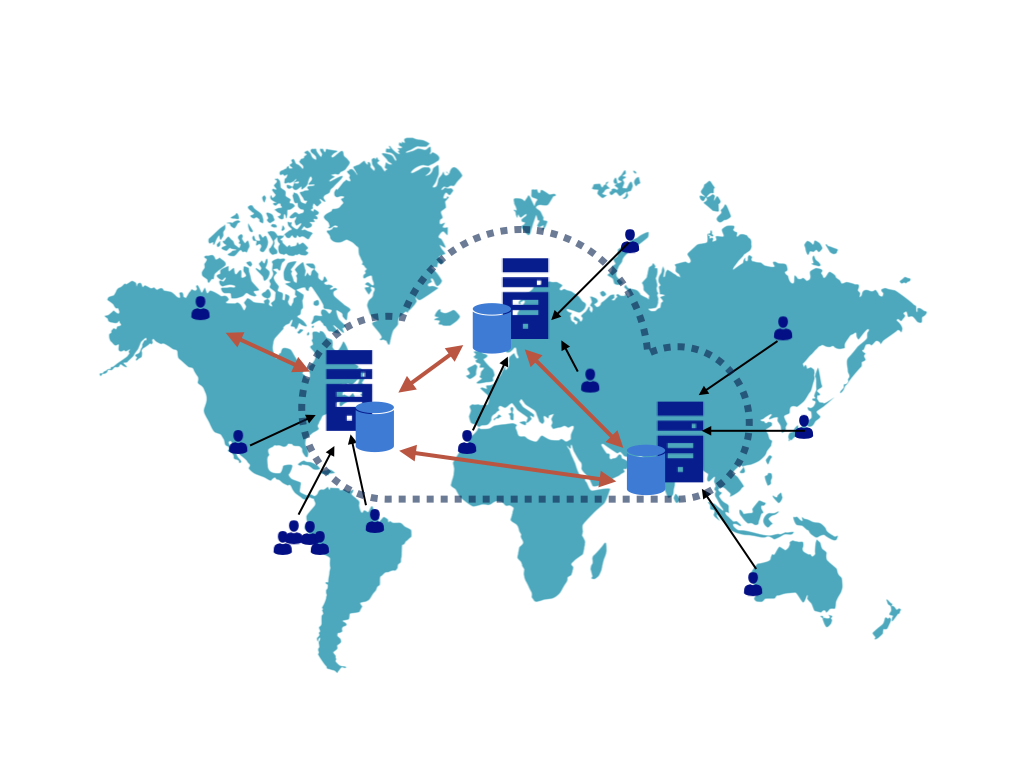
\includegraphics[scale=0.42]{figures/cloud-architecture.png}
    \caption{An example of the cloud computing model architecture, data is geo-replicated over three datacenters, which constitute the Cloud part of the system. The cloud benefits from a wired gygabit communication among them, illustrated by a red arrow. Client applications request data from the nearest datacenter replica, and only collaborate through the Cloud. Client to Cloud communication, illustrated by black arrows are usually slower.}
    \label{fig:cloud-architecture}
\end{figure*}

\section{Why Edge Computing?}
\label{ch:emergence-of-edge-computing}

We live in a world where smart devices are a large part of people's daily lives.
With the growing intelligence and computational capabilities of machines such 
as cars, phones, watches, home automation devices, augmented reality and 
various data sensors, 
it is becoming increasingly relevant to take advantage of the massive and 
ubiquitous resources of these smart devices.

\begin{figure*}[tph]
    \centering
    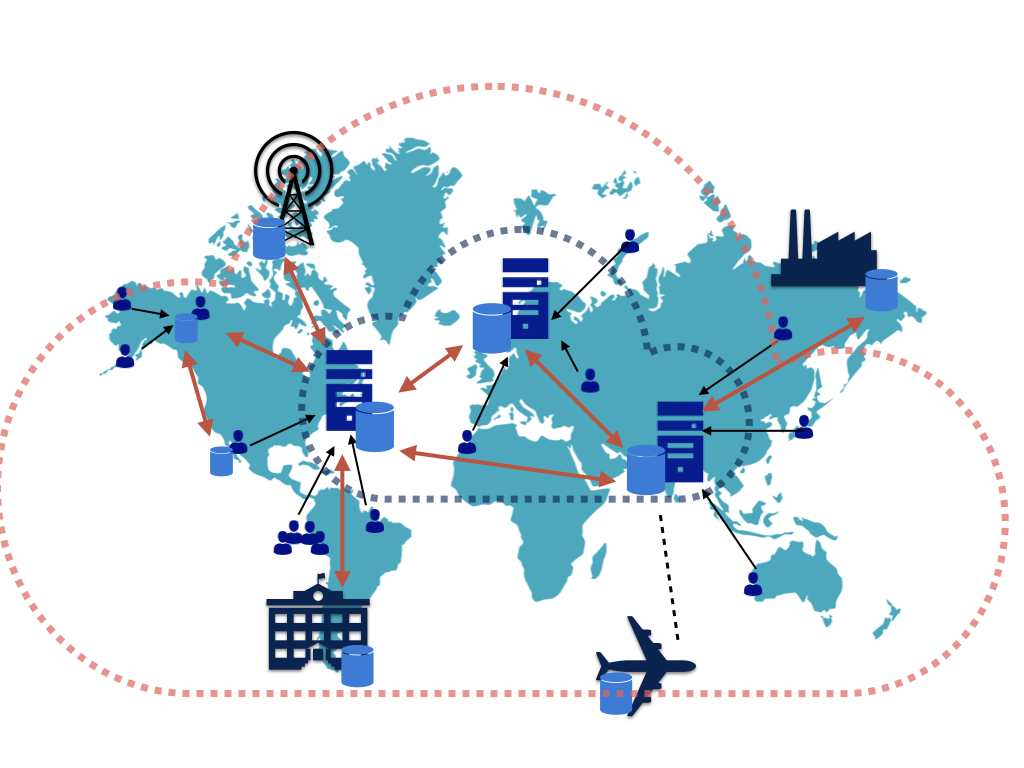
\includegraphics[scale=0.42]{figures/fog-architecture.png}
    \caption{An example of the Edge Computing model. The cloud model presented in figure~\ref{fig:cloud-architecture} is extended with new data replicas, closer to the users (i.e., the edge or the border of the network), this heterogeneous model mixes partial data replicas in a gigabyte wired school (high quality connections are illustrated with red arrows) or a manufacture company, a disconnected plane that will be reconnected after landing, users also store replicas in their own devices and can collaborate directly among them without the need to synchronize via the cloud server.}
    \label{fig:fog-architecture}
\end{figure*}

Data is increasingly produced at the network edge,
therefore, it would be more efficient to process data at the network Edge as 
well.
A cost study by Microsoft \cite{greenberg2008cost} shows that 
the traditional geo-distributed cloud design is less efficient than layered architectures at processing data when it 
is produced at the network edge.
In this context, 
the \textit{Fog Computing} model (depicted in Figure~\ref{fig:fog-architecture}), an emerging idea,
has been designed to provide a broader range of services by extending Cloud 
Computing to devices that deals with local data \cite{bonomi2012fog}.
The essence of the later proposal is that the majority (mote than 90\%) of raw data generated by IoT and stored at the cloud data center is arguably useless; in fact, it was observed that aggregates of data are often sufficient for most applications.

We define Edge Computing as a distributed architecture in which client data
is processed at the periphery of the network,
i.e., computation is done as close at to the originating end users as possible.
The concepts of fog and edge computing are expected to pave the way for a 
variety of possibilities for the future of intelligent embedded systems (IoT)
and the Internet.

Today's cloud computing technology has changed the way we use IT services
over the past decade.
It relies on the massive merging of computing and storage capabilities.
However, while cloud computing architecture excels at making internet services 
easier to use,
it also faces many obstacles.
Bandwidth limitations,
global centralization of data processing and storage have led to many
problems such as unwanted latency,
reduced mobility,
inability to be contextually aware,
and data synchronization overheads.
This is especially true for collaborative applications such as online gaming,
augmented reality and many other applications that require real-time 
analysis and control.

The emergence of edge-oriented computing paradigms,
such as fog/edge computing,
is no coincidence.
With the explosion in demand and growing dependence on fast information access 
and efficient data processing, 
edge-oriented computing paradigms have become an evolving necessity in the 
IoT (Internet of Things) domain.

Despite its growing popularity, 
putting edge-oriented computing into practice remains a challenge
\cite{shi2016edge}.
Fog and edge computing systems are still in the early stage of maturity.
Over the past few years, 
researchers have provided new and different perspectives on how these systems 
should be built.
There is no doubt that more effort is needed to realize the vision of fog/edge
computing.

\section{Network Architecture Challenges}
\label{sec:network-architecture-challenges}
Many proposals observe that edge applications offen generate
\cite{openfog1934ieee, sitton2019review}
large volumes of data at the edge of the network bu push it back to the 
cloud data centers for computation and 
storage.
This scenario has become increasingly prevalent with the exponential growth 
of the Internet of Things, 
where number of devices and consumed bandwidth are still increasing today
\cite{cisco2019visualnetworking}.
While the computing power of the cloud infrastructures can be adapted to the 
increasing pressure generated by IoT and other edge oriented applications,
the same cannot be said for the network infrastructures that connect IoT 
devices to the cloud \cite{shi2016edge, tarneberg2016experiences}, 
requiring measures and new technical contributions to,
on the one hand,
alleviate this load,
by delegating some computations to the system's edge,
and on the other hand,
allow their applications to operate with limited connectivity to the core.

A short-term solution \cite{bonomi2012fog} to this problem is to aggregate IoT
sensor data near the location (at the edge) where the data is generated, 
an idea that has been popularized by fog-based architectures and has been
widely adopted by industry \cite{yi2015survey}.
Unfortunately,
this approach does not address the fundamental problem of making these 
applications dependent on heavy computation (and storage) capabilities 
that are only available at the code in cloud infrastructures.
This observation is supported by the exponential growth of the IoT that is 
expected to continue for at least another decade, with predictions of more 
than a trillion totals connected and operating IoT devices by that time 
\cite{bol2019etictslides}. 
The massive amount of data that will be generated by these devices will require 
massive computing and storage capabilities to be continuously available,
which will not be possible by taking advantage of the core cloud infrastructures
alone.

Instead, a paradigm shift is needed to take advantage of the multiple layers of 
compute resources that exist between devices and cloud data centers by
decentralizing storage and computation.
Moving the components of these applications to the edge will effectively reduce
the amount of data that must traverse networks to reach data centers,
while allowing data to be processed closer to where it is generated,
improving quality of service,
namely faster response times,
for applications and the end users.

Another key challenge for edge and fog applications that is largely unaddressed
by the network and architecture literature and which we are interested 
int the background of this thesis is data management.
Data management is a non-trivial problem,
and dealing with it adequately at the application level places a nontrivial 
burden on application developers, which can lead to incorrect solutions.
In this thesis we will focus on this aspect of the state of the art,
and in particular on the availability and consistency aspects of data shared and
stored on different layers of the cloud-edge spectrum at the architectural 
level.

\section{Network Heterogeneity Challenges}
\label{sec:network-heterogeneity-challenges}
In edge computing,
the processing load should be distributed cooperatively across edge devices and cloud
servers.
Computation is distributed on each of these components depending on a number 
of factors, including network response time and the capacity of each node.

An edge network is typically composed of a large set of heterogeneous and loosely coupled compute nodes. 
An edge applications will frequently be exposed to several aspects that make 
their design and execution very challenging, namely high membership dynamics (nodes join, leave, and become unavailable), intermittent connectivity (network partitions), 
and weak communication order (messages are lost, duplicated or received out of order).

Many approaches have been proposed by the literature to classify 
heterogeneous devices in the Edge-Cloud networks \cite{ai2018edge}.
The main approaches being: Cloudlets \cite{satyanarayanan2009case} 
are computers or cluster of computers with above-average performance
and good connectivity to the internet;
MEC \cite{hu2015mobile} is an architecture for deploying a wide variety 
of applications on top of a host and is critical to the growth of the Internet
of Things (IoT);
For Computing \cite{bonomi2012fog} requires both the cloud and edge nodes 
and runs applications to meet a specific use case.

Fog Computing networks can include a mix of powerful and reliable nodes that
operate on data centers and small resource-limited and unreliable nodes that
operate at the edge.
Even among edge nodes,
there is considerable heterogeneity,
a laptop or a cell phone is much more powerful than other home automation 
IoT devices.
As different devices have 
different capabilities, 
it is unrealistic to expect full replication of the data that an 
application manages.

Network connections are also very heterogeneous and highly dynamic. 
Latency between edge nodes vary considerably, 
and some parts of the topology can be very dynamic while others are essentially 
stable. 
An algorithm that operates at the edge must account for this diversity and provide 
network reconfiguration protocols when necessary.

Finally,
the edge network suffers from \textit{churn} \cite{stutzbach2006understanding},
which consists of frequent changes in the operational state of network components.
Devices may connect or disconnect very frequently,
or even fail permanently.
As in the previous challenge,
additional solutions are needed to cope with these changes.

In this thesis, we distinguish three areas in the network.
The \emph{core} cloud is made of a few tens of resource-rich,
well-managed data centers (DCs).
At the opposite end of the spectrum, millions of resource-limited and
mismanaged \emph{far-edge} devices, such as mobile phones or IoT devices.
In between, thousands of \emph{border} nodes, such as CDN
Points-of-Presence (PoPs), metropolitan data servers, or 5G MEC servers.
We refer as ``edge'' to the union of the border and far edge, and as
``infrastructure'' to the union of the core and border.

\section{Data Management problem}
\label{sec:data-management-problem}
There is an increasing interest in the edge and fog computing paradigms 
aiming to reduce the dependency on cloud data centers.
While these paradigms bring several benefits on security, efficiency and 
cost, they incur new challenges nicely summarized in the eighth Pilars 
of the OpenFog Reference Architecture \cite{byers2017openfog}:
security, scalability, visibility, autonomy, reliability, agility, 
hierarchy and programmability.
Data management is a cross-cutting concern that touches most of these pillars,
it gathers all the mecanisms related to storage, data placement, access control
and privacy, and most importantly in this thesis data consistency.

At the same network area level (\textit{core, border} or \textit{far-edge}),
data management is mainly centralized,
most fog architectures does not provide data management directly among
lateral nodes.
A common pattern to share data in this case is to push it to a "parent" node
at a higher level.
The parent node plays a centralized data sharing role.
The existence of parent nodes reduces the autonomy, robustness,
and scalability of fog applications.

Across network area levels, data management is not consistent,
which means that applications cannot easily move from one fog level to another 
without violating correctness.
The consequence is that data management solutions have to be defined at 
each fog level.
Sometimes, to improve application responsiveness and reduce latency, 
loose synchronization patterns are used with loose consistency between fog levels.
If not carefully defined, 
these patterns introduce fundamental data inconsistency between fog levels, 
which greatly increases the complexity of creating and managing correct applications.

Solving these two problems would simplify collaborative applications 
development by addressing several requirements and properties,
specifically scalability, autonomy, availability, hierarchy and programmability.
The following sections will describe how the current systems addressed those
problems.

In fact, many distributed applications are currently designed to operate under strong consistency models, using solutions such as replicated state machines. This is due to the complexity of designing applications under weaker consistency models. Unfortunately, the use of these techniques is incompatible with the properties stated above. Therefore, there is a clear need to rethink how to develop distributed applications to work in edge computing environments.

There is currently no solution to easily develop and deploy applications within the edge computing paradigm. There is a lack of support for performing general-purpose computation in such a challenging environment. In particular, the current state of the art for performing computations on edge networks consists of gossip and peer-to-peer algorithms, which are capable of performing aggregate computations and providing immutable data content distribution across the edge network. Unfortunately, these techniques are still limited in scale and are not easily extended to support general computation on the edge, i.e., to perform any form of distributed computation on a shared, mutable state.

\section{Edge Storage Systems}
\label{sec:edge-storage-systems}
In the common case,
edge storage systems are designed for specific use cases \cite{byers2017openfog}
and not for general purpose.
This is due to the expected high volumes of traffic and the limited bandwidth 
of the cloud infrastructure.
Before data is transferred, there may be some pre-processing to reduce traffic 
or avoid it at all costs.
In addition, these storage systems choose lower consistency guarantees to 
reduce the storage and latency overhead associated with more powerful models.

One of the first caching systems, Cachier \cite{drolia2017cachier},
addresses recognition applications use case.
Most sample recognition algorithms operate in a pipelined mode and go through 
the following steps: 
feature extraction, feature classification and matching, 
and best match selection. 
They are computationally intensive, 
which does not allow them to run on edge nodes. 
As a compromise, these edge nodes can store parts of the model, 
so that they can be used to answer similar requests. 
This approach relies on the fact that clients in the same time and place request
similar things with a high probability. 
If a client requests something that cannot be satisfied by the cached model, 
the request is forwarded to the cloud, which responds with the result and the 
component responsible for obtaining it. The edge node sends the response to the 
client and caches the new component, 
following an initial LRU (Least Recently Used) policy that is modified over 
time. 
The main goal is to exploit a strategy that maximizes the number of times the 
edge node is able to respond to the client on its own.

Another situation is when the data needs to be archived,
but not all of it is interesting.
In another case \cite{ravindran2018edge},
the system monitors a region through video capture.
Since transferring all the images to the cloud requires huge network bandwidth 
and increases the latency of the analysis, the edge nodes run an algorithm to 
create feature vectors that allow relatively fast comparison between consecutive 
images. 
If two images have a similarity index above a predefined threshold, 
the differences are not significant and one of them can be discarded. 
Otherwise, the frame and its feature vector are time-stamped and tagged with a 
unique node identifier. 
Then it is placed in a transmission buffer to be sent to the cloud.

\section{Conclusion}
In this chapter, 
we introduced the edge computing model, its purpose and the problems related to its design.
We found that many scalability, efficiency and security challenges are induced 
to the edge network architecture and the heterogeneous ressources.
